\documentclass[12pt]{article}

%useful packages
\usepackage{color,soul}
\usepackage[usenames,dvipsnames,svgnames,table]{xcolor}
\usepackage{amsmath,amsthm,amscd,amssymb,bm}
\usepackage{hyperref}
\hypersetup{
    colorlinks=true,
    linkcolor=JungleGreen
}
\usepackage[utf8]{inputenc}
\usepackage[top=2cm, bottom=3cm, left=2cm, right=2cm]{geometry}
\usepackage{pgfplots}
\usepackage{enumitem}
\usepgfplotslibrary{fillbetween}
\usetikzlibrary{patterns}
\usepackage{tcolorbox}
\usepackage{centernot}
\usepackage{mathtools}
\usepackage{xcolor}

% Packages to create table 1
\usepackage{pdflscape}
\usepackage{subfig}
\usepackage{graphicx}


%personal definitions and commands
\newcommand{\R}{\mathbb{R}} 
\newcommand{\E}{\mathbb{E}}
\newcommand{\V}{\mathbb{V}}
\newcommand{\C}{\mathbb{C}}
\newcommand{\Prob}{\mathbb{P}}
\newcommand{\e}{\epsilon}
\newcommand\numberthis{\addtocounter{equation}{1}\tag{\theequation}} %allows numbering of single equations in align* environment
\newcommand{\mtx}[1]{\ensuremath{\bm{\mathit{#1}}}}
\newcommand{\B}{\hat{\boldsymbol{\beta}}}
\newcommand{\Cov}{\mathbb{C}\text{ov}}
\newcommand{\N}{\mathcal{N}}



\title{ECON675 -- Assignment 4}
\author{Anirudh Yadav}
\setlength\parindent{0pt}
\begin{document}

\maketitle

\setcounter{tocdepth}{2}
\tableofcontents

\newpage

\section{Estimating equations}

\subsection{Moment conditions}
The goal of this question is to show that the four given functions are valid moment conditions for the parameter $\theta_t(g)$. That is, we want to show that 
\begin{align*}
\E[\psi_{\texttt{f},t}(\mtx{Z}_i; \theta_t(g))] = 0,
\end{align*}
for each $\texttt{f} \in \{\texttt{IPW},\texttt{RI1},\texttt{RI2}, \texttt{DR}\}$. Note that in the derivations below I invoke LIE a lot without specifically mentioning it.\\

Start with the inverse probability weighting function
\begin{align*}
\E[\psi_{\texttt{IPW},t}(\mtx{Z}_i; \theta_t(g))] &=\E\left[\frac{D_i(t)\cdot g(Y_i(t))}{p_t(\mtx{X}_i)}\right] - \theta_t(g)\\
&=\E\left[\E\left[\frac{D_i(t)\cdot g(Y_i(t))}{p_t(\mtx{X}_i)}| \mtx{X}_i\right]\right] - \theta_t(g)\\
&=\E\left[\frac{1}{p_t(\mtx{X}_i)}\E\left[D_i(t)|\mtx{X}_i\right]\E\left[ g(Y_i(t))| \mtx{X}_i\right]\right] - \theta_t(g)
\end{align*}
Now, 
\begin{align*}
\E\left[D_i(t)|\mtx{X}_i\right] & = \Pr[D_i(t)=1|\mtx{X}_i] = \Pr[T_i = t|\mtx{X}_i] = p_t(\mtx{X}_i).
\end{align*}
Thus,
\begin{align*}
\E[\psi_{\texttt{IPW},t}(\mtx{Z}_i; \theta_t(g))] &= \E\left[\E\left[ g(Y_i(t))| \mtx{X}_i\right]\right] - \theta_t(g)\\
&=\E[g(Y_i(t))] - \theta_t(g)\\
&=0.
\end{align*}
Next, consider
\begin{align*}
\E[\psi_{\texttt{RI1},t}(\mtx{Z}_i; \theta_t(g))] &= \E[e_t(g;\mtx{X}_i)] - \theta_t(g)\\
&=\E[\E[g(Y_i(t)|\mtx{X}_i]] - \theta_t(g)\\
&=\E[g(Y_i(t)] -  \theta_t(g)\\
&=0.
\end{align*}
And,
\begin{align*}
\E[\psi_{\texttt{RI2},t}(\mtx{Z}_i; \theta_t(g))] &= \E\left[\frac{D_i(t)\cdot e_t(g;\mtx{X}_i)}{p_t(\mtx{X}_i)}\right]  - \theta_t(g)\\
&=\E\left[\E\left[\frac{D_i(t)\cdot e_t(g;\mtx{X}_i)}{p_t(\mtx{X}_i)}| \mtx{X}_i\right]\right] - \theta_t(g)\\
&=\E\left[\E\left[e_t(g;\mtx{X}_i)| \mtx{X}_i\right]\right] - \theta_t(g)\\
&= \E[e_t(g;\mtx{X}_i)] - \theta_t(g)\\
&=0.
\end{align*}
Finally, consider the doubly robust function
\begin{align*}
\E[\psi_{\texttt{DR},t}(\mtx{Z}_i; \theta_t(g))] &= \E\left[\frac{D_i(t)\cdot g(Y_i(t))}{p_t(\mtx{X}_i)}\right] - \theta_t(g) - \E\left[\frac{e_t(g;\mtx{X}_i)}{p_t(\mtx{X}_i)}(D_i(t)-p_t(\mtx{X}_i))\right].
\end{align*}
Using the IPW result above, we know that the first two terms cancel each other out, so that
\begin{align*}
\E[\psi_{\texttt{DR},t}(\mtx{Z}_i; \theta_t(g))] &=- \E\left[\frac{e_t(g;\mtx{X}_i)}{p_t(\mtx{X}_i)}(D_i(t)-p_t(\mtx{X}_i))\right]\\
&=- \E\left[\frac{e_t(g;\mtx{X}_i)D_i(t)}{p_t(\mtx{X}_i)}\right] + \E[e_t(g;\mtx{X}_i)]\\
&= -\theta_t(g) + \theta_t(g)\\
&=0.
\end{align*}
So each of the four functions is a valid moment condition for $\theta_t(g)$.

\subsection{Plug-in estimators}
The plug-in IPW estimator is 
\begin{align*}
\hat{\theta}_{\texttt{IPW},t}(g) = \frac{1}{n}\sum_{i=1}^n\frac{D_i(t)g(Y_i)}{\hat p_t(\mtx{X}_i)},
\end{align*}
where $\hat p_t(\mtx{X}_i)$ is the estimated propensity score. Note that since there are multiple treatment levels, the estimated propensity score would have to be computed using a suitable discrete choice model. For instance, $\hat p_t(\mtx{X}_i)$ could be estimated using a multinomial logit model.\\

The plug-in projection (or regression imputation) estimator is
\begin{align*}
\hat{\theta}_{\texttt{RI1},t}(g) = \hat{\E}[e_t(g;\mtx{X}_i)] =  \frac{1}{n}\sum_{i=1}^n \hat{\E}[g(Y_i(t))|\mtx{X}_i] &=  \frac{1}{n}\sum_{i=1}^n \hat{\E}[g(Y_i(t))|\mtx{X}_i, D_i(t)=1] \\
&= \frac{1}{n}\sum_{i=1}^n \hat{\E}[g(Y_i)|\mtx{X}_i, D_i(t)=1],
\end{align*}
where the second last equality uses the ignorability assumption. We need to make a choice about how to estimate the conditional expectation term. I think we could use NLS, or possibly a nonparametric method like kernel regression. To ease notation, let $\widehat{\mu}_t(\mtx{X}_i)$ be the parametric or nonparametric estimate of $\E[g(Y_i)|\mtx{X}_i, D_i(t)=1]$. Then, the projection estimator is
\begin{align*}
\hat{\theta}_{\texttt{RI1},t}(g) = \frac{1}{n}\sum_{i=1}^n \widehat{\mu}_t(\mtx{X}_i)
\end{align*}

The plug-in `hybrid' imputation estimator
\begin{align*}
\hat{\theta}_{\texttt{RI2},t}(g) &=  \frac{1}{n}\sum_{i=1}^n\frac{D_i(t)\widehat{\mu}_t(\mtx{X}_i)}{\hat p_t(\mtx{X}_i)}. 
\end{align*}
Finally, the plug-in doubly robust estimator is given by
\begin{align*}
\hat{\theta}_{\texttt{DR},t}(g) &= \frac{1}{n}\sum_{i=1}^n\frac{D_i(t)g(Y_i)}{\hat p_t(\mtx{X}_i)}-\frac{1}{n}\sum_{i=1}^n\frac{\widehat{\mu}_t(\mtx{X}_i)}{\hat p_t(\mtx{X}_i)}(D_i(t) - \hat p_t(\mtx{X}_i))\\
&=\frac{1}{n}\sum_{i=1}^n \left(\frac{D_i(t)(g(Y_i) - \widehat{\mu}_t(\mtx{X}_i))}{\hat p_t(\mtx{X}_i)} + \widehat{\mu}_t(\mtx{X}_i) \right).
\end{align*}
As discussed in Abadie and Catteneo (2018), the relative performance of the above estimators depends on the features of the data generating process. In finite samples, IPW estimators become unstable when the propensity score approaches zero or one and regression imputation estimators may suffer from extrapolation biases. Doubly robust estimators include safeguards against bias caused by misspecification but impose additional specification choices that may affect the resulting estimate.

\subsection{Estimating the variance of potential outcomes}


\newpage
\section{Estimating average treatment effects}

Estimation results are overleaf. Estimates of ATEs are very different across the Lalonde and PSID control samples (for all estimators), which suggests that there are large and systematic differences between the two control groups . For instance, ATEs are generally positive when using the Lalonde control, while many ATEs are large and negative when using the PSID control group. This makes sense because the NSW program was targeted at individuals who had faced economic and social problems prior to enrolment (i.e. these respondents, on average, had low incomes), whereas the PSID sample is more representative of the entire US population. \\

Most estimates of ATTs are broadly similar across the samples. The ATTs using matching estimators are quite similar across both samples. Again, this makes sense, because matching estimators specifically ensure that there is a decent degree of covariate balance between the treatment and control samples (i.e. the matching estimators would pick respondents from the PSID sample who have similar characteristics to the respondents in the Lalonde experiment).\\

I had some issues with the estimation of both ATEs and ATTs:
\begin{itemize}
\item I had problem getting RI/IPW/DR estimates for PSID covariate set A in \verb|R| (using the \verb|CausalGAM| package) so I used \verb|STATA| only in this case.
\item IPW and DR ATT estimates are the same in \verb|STATA|; I'm not sure why.
\item Many of the logit regressions for estimating propensity scores did not converge, so I generally set the maximum number of iterations to 25.
\end{itemize}



\begin{landscape}
\begin{table}
\centering
\caption{Estimation and Inference on ATE and ATT}\label{tab:tableQ2}
\vspace{-.1in}\resizebox{\columnwidth}{!}{
\subfloat[][ATE]{\input{teffectsATEq.txt}}\quad
\subfloat[][ATT]{\input{teffectsATTq.txt}}
}
\end{table}
\end{landscape}

\newpage

\section{Post-model selection inference}

\subsection{Summary statistics and density plots}
The summary statistics for each estimator are presented in Table 2 and the kernel density plots are just below. As expected, the empirical distribution of $\hat{\beta}$ is approximately normal and the distributions of $\tilde{\beta}$ and $\check{\beta}$ are not.

\begin{table}[!htpb]
\centering
\caption{\textbf{Summary Statistics for each Estimator}}
\begin{tabular}{crrrrrr}
  \hline
Estimator & Min. & 1st Qu. & Median & Mean & 3rd Qu. & Max. \\ 
  \hline
(i) $\hat{\beta}$ & -0.50 & 0.32 & 0.52 & 0.51 & 0.71 & 1.32 \\ 
(ii) $\tilde{\beta}$ & 0.77 & 1.26 & 1.36 & 1.36 & 1.47 & 1.88 \\ 
(iii) $ \check{\beta}$& -0.50 & 0.32 & 0.52 & 0.54 & 0.72 & 1.66 \\ 
   \hline
\end{tabular}
\end{table}

\begin{figure}[!htpb]
    \centering
    
        %\centering
        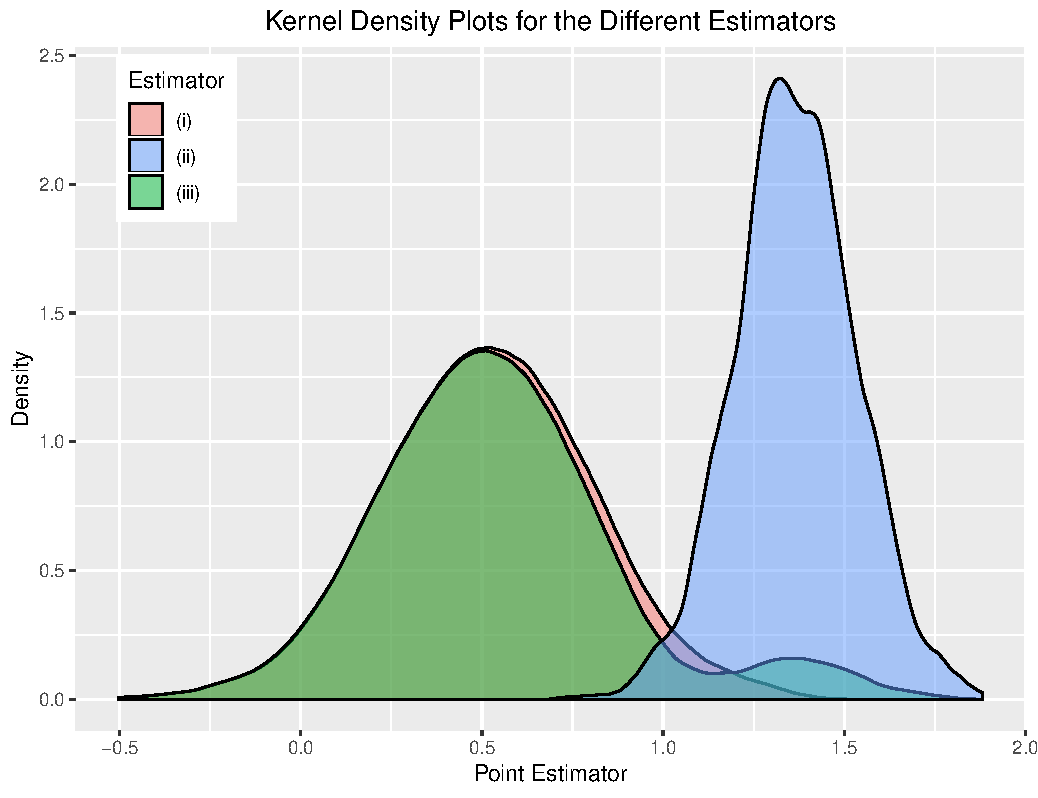
\includegraphics[width=0.7\textwidth]{dens.pdf}

\end{figure}

\end{document}
